\documentclass{acm_proc_article-sp}
\RequirePackage[T1]{fontenc}
\usepackage[cp1250]{inputenc}

\usepackage{pgf}
\usepackage{tikz}
\usepackage{listings}
\usepackage{url}
\usepackage{xspace}
\numberofauthors{3}
\author{
\alignauthor
J�drzej Fulara\\
\affaddr{Institute of Informatics}\\
\affaddr{University of Warsaw}\\
\affaddr{ul. Banacha 2}\\
\affaddr{02-097 Warsaw, Poland}\\
\email{fulara@mimuw.edu.pl}
\alignauthor
Krzysztof Jakubczyk\\
\affaddr{Institute of Informatics}\\
\affaddr{University of Warsaw}\\
\affaddr{ul. Banacha 2}\\
\affaddr{02-097 Warsaw, Poland}\\
\email{kjk@mimuw.edu.pl}
\alignauthor
Aleksy Schubert\\
\affaddr{Institute of Informatics}\\
\affaddr{University of Warsaw}\\
\affaddr{ul. Banacha 2}\\
\affaddr{02-097 Warsaw, Poland}\\
\email{alx@mimuw.edu.pl}
}
\bibliographystyle{abbrv}
\title{Supplementig Java Bytecode with Specifications}

\newcommand{\jmltobmltext}{JML2BML}
\newcommand{\jmltobml}{\textsl{\jmltobmltext}\xspace}
\newcommand{\openjml}{OpenJML\xspace}
\newcommand{\bmllib}{BMLLib\xspace}
\newcommand{\hs}{\hspace{0.5pt}}


\lstdefinelanguage{BML}{morekeywords={abstract,break,byte,case,catch,char,class,%
      const,continue,default,do,double,else,extends,false,final,%
      finally,float,for,goto,if,implements,import,instanceof,%
      interface,label,long,native,new,
      boolean, int,%
      null,%
      package,private,protected,public,ghost,%
      return,short,static,super,switch,synchronized,this,throw,%
      throws,transient,true,try,void,volatile,while,
      requires,precondition,ensures,exsures,exists,forall,&&,%
      old_this,loop_inv,\result,\everything,\nothing,%
      loop_specification,modifies,invariant,decreases,%
      iconst_0,iconst_1,istore_3,iinc,iload_3,%
      aaload,aload_0,aload_1,aload_2,aastore,%
      if_acmpne,if_icmplt,%
      invokespecial,getfield,%
      arraylength,ireturn},%
   sensitive,%
   morecomment=[l]//,%
   morestring=[b]",%
   morestring=[b]',%
    basicstyle=\small,
    keywordstyle=\bfseries\color{black},
    commentstyle=\itshape\color{blue},
    mathescape=true,
}


\begin{document}
\maketitle


%\section{What should be in paper}
%\begin{itemize}
%	\item What is JML
%	\item What is BML
%	\item Why is translation needed??
% \item Why the tool needed?? (JVM -> VM) BML can be used to different languages, JML to one??
%	\item The tool isn't built on any existing comipler.
%	\item As input we get source file with JML annotations and compiled class file.
%	\item Therefore we can't used optimised bytecode (problem with loops, assertions etc.)
%	\item Optimized bytecode may be used for more general annotations eg. method invariants.
%	\item Detecting loops in bytecode
%	\item Description of matching source code with bytecode loops
%	\item Non-trivial example
%\end{itemize}
\maketitle
\begin{abstract}
Java class file is an interoperable format that can serve not only to
transfer the compiled versions of Java programs, but also to embed
into the files additional information which can be exploited by the
execution environment of user's machine to speed up the execution of
the application or to ensure certain vital properties of the code. The
latter goal is specifically the aim of the proof-carrying code (PCC)
techniques in which the executable code is supplied with a proof that
the code obeys certain policy (e.g. the program does not store
password cleartext in a file). BML (Bytecode Modelling Language) can
be regarded as a part of the PCC architecture which allows to express
detailed properties of bytecode programs, in particular the policies
they must obey.

As most of the programming is done at the source code level, it is
desirable to have a way to translate properties expressed at the
source code level (in our case written in Java Modeling Language, JML)
to the bytecode level.  In this paper we present a \jmltobml
compiler, a tool that for a given Java source file annotated with
specifications generates class files with BML.
\end{abstract}
%# Alternative languages on the Java VM
%# Java Extensions
%#  - PCC
%#  Optimization
%#  - PCC
%# VM Design
%# Java Verification
%#  - PCC
%#Java for Embedded Systems
%*   Middleware for Mobile Applications
%* Location-Based Services
%* M-Business Applications
% page limit: 10 pages

\category{D.2.4}{Software Engineering}{Software/Program Verification}

\terms{Reliability, Verification}

\keywords{Java, byte code, JML, BML} % NOT required for Proceedings

\section{Introduction}

Each Java Virtual Machine is required to perform so called bytecode
verification process on each class file which is loaded to be executed
\cite{verification}. This verification process ensures vital
properties of the loaded programs such as that all arguments on the
operand stack are legal, all types of variables passed to methods are
correct, all load and store operations have correct types, etc.

In certain situations, these guarantees are not sufficient. In
particular, many of the current security guarantees are ensured at
runtime of an application. For instance, a mobile application asks the
user to acknowledge the sending of data over the mobile
network. However, the user may get bored with many such prompts and
disable this security property. After this, she or he may easily be
made to send data to e.g. an expensive premium number. In this case,
it would be more secure to give the user a load- (or download-) time
guarantee that the code sends data only to expected receivers.
Currently, this is partially done through digital signatures. The
signatures, however, do not assure that the software is indeed
secure. They only certify who takes (not so well defined)
responsibility for the problems caused by the program.  In fact, there
were cases when many users were deceived by respected companies
e.g. rootkits were installed when audio CD was inserted \cite{BMGcase}.

Another guarantee which is not secured by the traditional bytecode
verification procedure is the lack of code inconsistencies typically
considered to be programming errors i.e. null-pointer exceptions,
array index out of range exceptions etc. In many cases, these
inconsistencies can be eliminated with the help of some additional
information (e.g.@NonNull annotations, suggested in \cite{JSR305})
which makes the checking process feasable.

The presence of traditional bytecode verification enables certain
speed-ups at the run time. In particular, the method invocation
instruction need not check the type of the object on which the method
is invoked. The more detailed information we have the more
optimizations we can introduce. For instance the credible information
on the value of an array index may release the array access bytecode
instructions from the checks that the access is within the available
region \cite{SafeUntrusted98}.

The goal of the proof-carrying code (PCC) technique
\cite{pcc,AScalable} is to give the user certain guarantees of the
code to be executed at the moment of its execution. In this paradigm,
the executable code (in case of Java, the bytecode) is augmented with
an additional piece of information, a PCC certificate, which together
with the code makes possible an automatic check that the code indeed
obeys the expected policy (e.g. sends data to authorised targets
only). This check is performed by the user (or by user's execution
environment) right before the code is executed (see
Figure~\ref{fig:pccScheme}). In fact, the usual Java bytecode
verification procedure can be viewed as an example of a forerunner of
thich technique. Although the certificate is in this case empty (or
supplementary in case the StackMap attributes are employed), the
execution environment indeed checks a vital code property before the
code is executed. In more complicated cases of the proof-carrying
code, one needs the additional information to make the checking of the
required property feasible or even algorithmically possible.

One of the possible ways to realise the PCC architecture is developed
under the european project MOBIUS.\footnote{See
\url{http://mobius.inria.fr}} This project plans to develop both
type-based and logic-based PCC program certification techniques
\cite{MOBIUSscenarios}. The logic-based methods rely on specification
of the object-oriented code in the fashion governed by the
design-by-contract principles \cite{DesignByContract}. Bytecode
Modeling Language (BML) is a specification language which realises the
methodology at the bytecode level \cite{bmlBurdy}. It is designed as a
counterpart of the Java Modeling Language (JML), an established
specification language dedicated to formally describe properties of
Java programs in the design-by-contract style \cite{JML}.

\begin{figure}
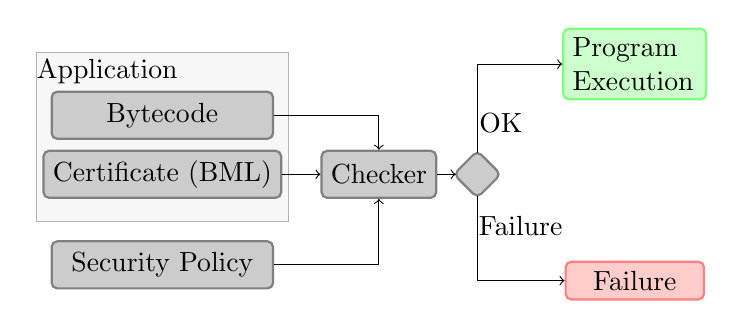
\begin{tikzpicture}[scale=0.5]

\tikzstyle{vertex}=[rectangle,draw=black!50,fill=black!20,thick,rounded corners = 2pt, minimum width=80pt, minimum height=17pt]
\tikzstyle{vertex2}=[rectangle,draw=black!50,fill=black!20,thick,rounded corners = 2pt, minimum height=17pt]
\tikzstyle{vertex3}=[rectangle,draw=green!50,fill=green!20,thick,rounded corners = 2pt, minimum width=50pt, text width=45pt]
\tikzstyle{vertex4}=[rectangle,draw=red!50,fill=red!20,thick,rounded corners = 2pt, minimum width=50pt]

\tikzstyle{rotated}=[rectangle,draw=black!50,fill=black!20,thick,rounded corners = 2pt,rotate=45, minimum height=12pt, minimum width = 12pt]
\tikzstyle{rl}=[line join = round]
\filldraw[draw=black!30,fill=black!3] (-3.2,3.8) rectangle (3.2,-0.5);
\node (app) at(-1.4,3.3) {Application};
\node[vertex] (bytecode) at (0,2.2){Bytecode};
\node[vertex] (certificate) at (0,0.7) {Certificate (BML)};

\node[vertex](policy) at (0, -1.6) {Security Policy};

\node[vertex2](checker) at (5.5,0.7) {Checker};
\node[rotated](rot) at (8, 0.7) {};
\node[vertex3](execution) at (12,3.5) {Program Execution};
\node[vertex4](failure) at (12,-2) {Failure};
\draw[->] (certificate) to[out=0,in=180] (checker);
\draw[->] (checker.east) -- (7.45,0.7);
\draw[->] (bytecode.east) -- (5.5,2.2) -- (checker.north);
\draw[->] (policy.east) -- (5.5,-1.6) -- (checker.south);
\draw[->] (8,1.25) -- (8,3.5) -- (execution.west);
\draw[->] (8,0.15) -- (8,-2) -- (failure.west);
\node (ok) at (8.6, 2) {OK};
\node (ok) at (9.1, -0.6) {Failure};
\end{tikzpicture}
\caption{Proof-Carying Code architecture for bytecode.}
\label{fig:pccScheme}
\end{figure}

The use of specification formalisms such as JML or BML has another
important application. Modern, high level programming languages
support creating software in a modular way. Applications can be
divided into smaller parts that can be developed independently. In
large systems, it is a common practice to outsource some well defined
subsystems to external companies. The main problem in this approach is
that the pieces of software developed by different programming teams
often are not fully compatible. To avoid this incompatibility and
useless code that is produced, there is a need to specify precisely
the desired behaviour of the components, what they require and what
can we expect from them \cite{SoftwareReuse}. The solution is to
define formally implementation contracts in languages such as JML or
BML and check automatically the compliance of the code with these
descriptions.

Specification languages are useful in describing the system components
behaviour. They are not only helpful in dividing the problem into
smaller pieces, but also focus on \textit{what} is expected from each
part, without saying about \textit{how} should it be done. The
specification languages are designed to be simple enough to be
understood by programmers, so they can play role of code
documentation. Using specification language for documenting code has
the advantage that it is possible to automatically verify that the
source code implements the documented features
\cite{formalDocumentation}.

The distributed development of software results in a situation where
different software modules are implemented in different
languages. This is facilitated by the fact that more and more
languages are compiled to the same Java bytecode. A few examples:
\begin{itemize}
\item Jython: the Python Java implementation,
\item JRuby: the Ruby Java implementation,
\item Jacl: the Tcl Java implementation,
\item Rhino: the JavaScript Java implementation,
\item Scala: a functional programming language compiled to
  Java bytecode.
\end{itemize}
At SugarCon 2008, Sun Microsystems President and CEO Jonathan Schwartz
said "we are just going to take the 'J' off the 'JVM' and just make it
a 'VM'". Therefore there will be a global trend with support of
companies to use JVM with languages other than Java.  This is an
important reason, why it is important to be able to translate the
source code specifications into lower level language
specifications\hs{}---\hs{}in case the development is done in many
languages the only common platform is the platform of the executable
code. This explains the efforts concerning BML specification language.

The JML specification language exists already for several years. In
the course of the time, a lot of code have been annotated with the
specifications in this language (see \cite{overviewOfJML} for an
overview). Except for that, it is easier to understand and specify the
code in the source form than in the bytecode form. In this light, it
is desirable to translate these specifications from JML to
BML. Moreover, the code producer in PCC scenarios, who has to produce
a correctness proof, will often prefer to construct it rather in terms
of the source code than in terms of the bytecode, and then compile the
specification and the proof into the level of executable code.

In a broader perspective, the full infrastructure to support the use
of BML annotated programs, for which complicated properties are
checked at the user's end, requires the following items:
\begin{itemize}
\item PCC checker tools that understand BML annotations combined with
  PCC certificates,
\item tools which enable the construction of PCC certificates,
\item procedures to safely distribute the desired properties to be
  checked by PCC infrastructure,
\item modelling languages (such as JML for Java) for other programming
  languages,
\item compilers that compile programs to JVM bytecode along with
  annotation compilers,
\end{itemize}
The \jmltobml compiler described in this paper is designed to be a
part of this scheme which translates the policies and specifications
to the bytecode format.

\paragraph{Organisation of the paper}
In Section~\ref{sec:specification}, we present the specification
languages JML and BML. An example which illustrates the work of the
compiler is presented in Section~\ref{sec:example}.
Section~\ref{sec:compiler} overviews the design of the \jmltobml
compiler. The most difficult problem of the specification compilation
is the placement of the loop invariants. This issue is discussed in
Section~\ref{sec:loops}. The related work is presented in
Section~\ref{sec:related-work} and we conclude in
Section~\ref{sec:conclusion}.


\section{Specification Languages}
\label{sec:specification}

\subsection{JML}
The Java Modelling Language (JML) is a behavioural specification
language for Java prigrams \cite{JML}. It allows to write
specifications according to the \textit{design-by-contract} principles
\cite{DesignByContract}. Data types and method behaviour can be
precisely commented using JML annotations. They describe the invariant
properties that are maintained by objects, the input method
requirements (preconditions), what we can expect at the output of
method (postconditions) and also some lower level properties of the
code (i.e. loop invariants, loop variants etc). JML annotations are
written in standard Java comments, so they do not affect the normal
work of any Java compiler.

An important goal in the design of JML is that it should be easily
understandable by Java programmers. It is achieved by staying as close
as possible to the Java syntax and semantics. The tool support for JML
is rich (see \cite{overviewOfJML} for an overview). In particular,
there are tools that check JML specification at runtime
\cite{runtime}, in extended static checking fashion \cite{escJava},
and allow to perform software certification \cite{krakatoa}. There are
also tools that support annotation generation
\cite{canapa},\cite{daikon}.

The works on JML was started by Gary Leavens at Iowa State
University. Since then it became an open project, multiple groups
around the world are writing tools supporting JML and developing the
language itself.

\subsection{BML}
The Bytecode Modelling Language (BML) is a specification language for
the bytecode. It was proposed by Burdy et al. in \cite{bmlBurdy}. The
design of BML directly follows the fundamental concepts of JML. It
inherits most constructs and keywords from the JML syntax. As the
BML is developed within the MOBIUS \cite{mobius} project and the main
target of the project are Java-enabled mobile devices such as mobile
phones, the current version of BML assumes some simplifications of the
Java bytecode which are present in the J2ME platform\hs{}---\hs{}the Java
platform for mobile devices with restricted resources.

The class files representing bytecode with BML annotations are regular
Java class files, executable by all Java tools. The annotations are
stored within additional attributes. The BML related attributes start
with the prefix \texttt{org.bmlspecs} and according to the
specification of the Java Virtual Machine they should be ignored by
the Machine, since their names are not part of the original JVM
specification.

Of course, following the logical structure of class files, class
specifications are stored as class attributes, method specifications,
as attributes of corresponding method and specifications inserted in
the code are attributes of the JVM Code attribute of the given method.

\subsection{Overview of annotations}

The structure of annotations in BML and JML is very similar. We have
two main types of annotations: method annotations and data type (class
and interfaces) annotations.

\subsubsection{Method annotations}
The most important type of method annotations are \textit{method
specifications} describing the input-output behaviour of the
method. These are preconditions (\texttt{requires}), defining
conditions that should be fulfilled before entering the method and
postconditions (\texttt{ensures}) telling what we can expect after the
method finishes. One can define also which fields are modified (clause
\texttt{modifies}) and which exceptions might be thrown (clause
\texttt{signal}).

The other type of method annotations are specifications elements
appearing in the code. These include:
\begin{itemize}
\item {Assert instructions that state some facts about fields,
  variables etc. that should hold at this point of program execution.}
\item {Loop specifications that describe the loop invariants
  (\texttt{loop\_invariant}) that describe the operation of the loop,
  loop variants (\texttt{decreases}) that explain why the loop
  terminates, and frame conditions (\texttt{modifies}) that tell which
  fields or variables can be changed in this loop.}
\item{Declarations of local \texttt{ghost}
  variables\hs{}---\hs{}variables that exist only in the
  specification. Their values can be modified only using special
  \texttt{set} instructions. These variables are used as shorthands
  for certain definitions as well as a means to capture the
  information flow properties within the specified program.}
\item{\texttt{Set} instructions that allow to modify ghost fields and
  variables.}
\end{itemize}

\subsubsection{Data type annotations}
Class (and interface) specifications describe the behaviour of a class
as a whole (in the \texttt{static} version) or of objects of that
class (\texttt{instance}). The most important type of \textit{class
specifications} are class invariants. They describe the property that
should hold for all objects of this class in all \textit{visible}
states, i.e. after all constructors and before and after all
methods. For example, having a field \texttt{Object[] list}, one can
write an invariant that the list is never null and its length is
10. Class invariants can be seen as additional, implicit preconditions
and postcondtitions for all methods in the class.

Other important class specifications are:
\begin{itemize}
\item {Declarations of \texttt{ghost} fields. They are similar to
  local ghost variables, but are visible in the whole class scope.}
\item {Model fields\hs{}---\hs{}fields present only in the specifications,
  representing some more complicated formulas. For example one can
  create a model field representing the property that a collection does
  not contain nulls.}
\end{itemize}
More details can be found in \cite{jmlrefman} and \cite{bmlrefman}.

\lstset{language=java, morekeywords={requires,ensures,\result,\exists,\old,loop_invariant,\forall,==>, decreases},
        basicstyle=\scriptsize,commentstyle=\scriptsize,moredelim=*[s][\scriptsize]{/*@}{*/},
        numbers=left,numberstyle=\tiny,stepnumber=4,numbersep=5pt}
\begin{figure}[htbp]
~~~~~~%
\begin{minipage}{400pt}
\begin{lstlisting}
public class List {

  private Object[] list;

  /*@ requires list != null;
    @ ensures \result ==(\exists int i;
    @ 0 <= i && i < list.length &&
    @ \old(list[i]) == o1 && list[i] == o2);
    @*/
  public boolean replace(Object o1, Object o2){
    /*@
      @ loop_invariant i <= list.length
      @ && i >=0 && (\forall int k;0 <= k
      @ && k < i ==> list[k] != o1);
      @ decreases list.length - i;
      @*/
    for (int i = 0; i < list.length; i++) {
      if (list[i] == o1) {
        list[i] = o2;
        return true;
      }
    }
    return false;
  }
}
\end{lstlisting}
\end{minipage}
\caption{An example class \texttt{List.java} containing single method \texttt{replace}.}
\label{fig:source}
\end{figure}

\section{An Example of Using The\\Compiler}
\label{sec:example}

This section provides an example demonstrating the result of launching
the \jmltobml.
\subsection{Source code}
Consider the class presented on Figure~\ref{fig:source}. This is an
excerpt of a class which implements a sequence of objects. We present
here only one method that replaces in the \texttt{list} array the
first occurence of its first parameter with the second one. True will
be returned, if and only if such an element was found.

The presented code, apart from standard Java statements, contains also
specifications in the JML. The specifications are embodied within
special Java comments starting with \verb!/*@! and ending with
\verb!@*/!. The precondition for the method \texttt{replace} starts
with the keyword \texttt{precondition}. It requests that every time
the method is invoked, the field \texttt{list} it not
\texttt{null}. In practice, the precence of such a precondition means
that JML tools will warn the programmer each time she or he tries to
use the replace method and the non-nullness of the \texttt{list} field
cannot be guaranteed.

The precondition line is followed by a line starting with
\texttt{modifies} keyword. This line specifies which variables can be
changed in the course of the method execution. The specification on
Figure~\ref{fig:source} tells that the method can change any value. In
certain situations (e.g. sometimes we can omit synchronisation when
the method only reads information), it is useful to have more detailed
knowledge concerning the modifications performed by the method.

The next three lines (starting with \texttt{ensures}) constitute the
method postcondition. It states that, if the precondition is
fullfiled, then the method result is true if and only if there is an
slot in the \texttt{list} the value of which has been updated from
\texttt{o1} to \texttt{o2}. Note that the postcondition makes use of
special JML expressions such as \texttt{$\backslash$result} (which
denotes the result of the method), \texttt{$\backslash$old} (which
allows to refer to a value of expression rather at the moment of the
method invocation than at the exit) or \texttt{$\backslash$exists}
(which allows to express the existential quantification). This
postcondition does not describe full requirements concerning the
method. For example an implementation that replaces all elements in
the \texttt{list} up to the first occurence of \texttt{o1} with
\texttt{o2} would fulfill this specification. However, it is not
difficult to provide more accurate property.

In additition to specifications describing input-output behaviour of
the method, a formal description of the loop implementing the
\texttt{replace} method is provided. The first part of the description
is the \texttt{loop\_invariant} clause which contains a loop
invariant: a formula that should hold at the beginning of the loop
body in each its iteration. In this example, it states that in
iteration \texttt{i} there are no occurences of \texttt{o1} in
\texttt{list} on positions before \texttt{i}. The second loop
annotation is \texttt{decreases}clause which describes the loop
variant. It specifies an expression (in this case
\verb|list.length - i|) the value of which strictly decreases in each
loop iteration.

\subsection{Bytecode}
In this section we describe the result of translating the source code
from Figure~\ref{fig:source}. Since the binary class files are not
easily readable, we rely on their textual representation obtained from
the \bmllib library. In case there are no annotations, the textual
representation is just the textual representation returned by Byte
Code Engineering Library (BCEL) and is similar to the output of
\texttt{javap} tool or the input acceptable by Jasmine language
\cite{Jasmin}. The Figure \ref{bytecode} shows the translated
\texttt{replace} method together with BML annotations inserted by our
\jmltobml compiler. Lines 0 and 1 correspond to the initialization
\texttt{i = 0}. The loop is located between lines 2 and 33. Lines
5--12 represent the \texttt{if} statement, 15--23 correspond to lines
??? from the source code. Loading loop condition parameters is located
in lines 27--32 and 33 performs the loop condition comparison.

The \texttt{requires-enusers} pair is translated into input-output
behaviour BML specifications located just before the method
code. Loops specifications are located after line 32 in the presented
listing. The \jmltobml compiler detects loops in the bytecode and
inserts the annotation before the statement representing the loop
condition. In this case it is the \texttt{if\_icmplt} instruction
comparing \texttt{i} and \texttt{list.length}. For more details about
detecting loops refer to Section~\ref{sec:loops}. The modifies clause
describes set of variables modified by the loop. Currently, because of
\openjml limitations it is not supported by our compiler (the default
value \texttt{$\backslash$everything} will be inserted).

\section{\jmltobmltext{} Compiler Design}
\label{sec:compiler}

In our work we have designed and implemented a tool called
\jmltobml that compiles JML specifications into BML. It takes
as input a Java source file with JML annotations, the corresponding
class file and outputs the class file with inserted proper BML
annotations. Our compiler uses an enhanced Abstract Syntax Tree for
the Java source code, taken from the \openjml compiler. For
different types of JML clauses, there are separate translation rules
defined. At each node of the AST, all translation rules are
applied. If some rule succeeds to translate this node, the result is
stored in to the class file, using the \bmllib library
\cite{bmllib}. This approach makes the compiler easily extensible. One
can simply write new translation rule to support additional features
of the JML language.

Currently the \jmltobml compiler focuses on subset of the JML
called JML Level 0. Due to external libraries limitations not all
desired features are translated, for example the
\texttt{loop\_modifies} clause is not supported by the
\openjml.

The \jmltobml is designed to be compatible with other bytecode
level tools, such as the bytecode editor \textit{Umbra}.

\subsection{Architecture description}
In this section we present the overview of the architecture of \jmltobml
compiler. The \jmltobml compiler uses \openjml to parse
the Java source code together with the JML annotations. To insert
generated BML annotations, the \bmllib library is used. The
dependencies between internal packages of \jmltobml and
\openjml and \bmllib are presented in Figure
\ref{packages}.

\begin{figure}[htbp]
\lstset{language=bml}
\lstset{basicstyle=\small}
~~~~~~%
\begin{minipage}{400pt}
\begin{lstlisting}
/*@
  @  \precondition list != null
  @  \modifies \everything
  @  \ensures \result ==
  @    (\exists int i; 0 <= i && 
  @        i < this.list.length &&
  @        old_this.list[i] == o1 &&
  @        this.list[i] == o2)
  @*/
public boolean replace(Object o1, Object o2)
0:    iconst_0
1:    istore_3
2:    goto	   #27
5:    aload_0
6:    getfield	   main.List.list
9:    iload_3
10:   aaload
11:   aload_1
12:   if_acmpne	   #24
15:   aload_0
16:   getfield	   main.List.list
19:   iload_3
20:   aload_2
21:   aastore
22:   iconst_1
23:   ireturn
24:   iinc	   %3	1
27:   iload_3
28:   aload_0
29:   getfield	   main.List.list
32:   arraylength
/*@
  @\loop_specification
  @  \modifies \everything
  @  \invariant i <= list.length &&
  @     i >= 0 &&
  @     (\forall int k; 0 <= k &&
  @         k < i ==> list[k] != o1)
  @  \decreases list.length - i;
  @*/
33:   if_icmplt	   #5
36:   iconst_0
37:   ireturn

\end{lstlisting}
\end{minipage}
\label{bytecode}
\caption{The method \texttt{replace} in the \texttt{List.class}}
\end{figure}

The \texttt{jml2bml.main} package provides the entry point to the
application. JML annotations from given source file will be translated
and inserted into corresponding \texttt{class} file. Functions to
access some bytecode information are located in
\texttt{jml2bml.bytecode} and helpers to \bmllib are collected
in \texttt{jml2bml.bmllib}. The \texttt{jml2bml.rules} package
contains translation rules for different aspects of JML. It should be
easy to add new rules in the future. Classes for traversing the Java
abstract syntax tree can be found in \texttt{jml2bml.ast}. In
\texttt{jml2bml.symbols} implementation of symbol table can be
found. The \texttt{jml2bml.engine} package contains the core
translating mechanism.
\begin{figure}[h]
\centering{
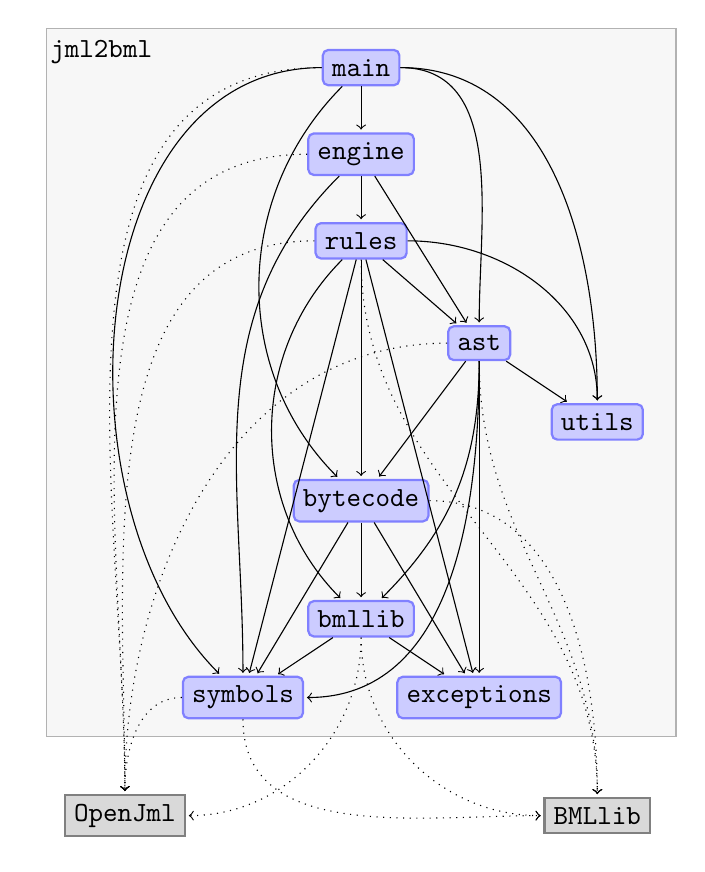
\begin{tikzpicture}[shorten >=1pt,->]
\
\tikzstyle{vertex}=[rectangle,draw=blue!50,fill=blue!20,thick,rounded corners = 2pt]
\filldraw[draw=black!30,fill=black!3] (-1,7.5) rectangle (7,-1.5);
%\draw (-0.9,7.2) node[right]{\textbf{\texttt{jml2bml}}};
\node (label) at (-0.3,7.2){\texttt{jml2bml}};
\node[vertex] (main) at (3,7) {\texttt{main}};
\node[vertex] (engine) at (3,5.9) {\texttt{engine}}  ;
\node[vertex] (rules) at (3,4.8) {\texttt{rules}}  ;
\node[vertex] (ast) at (4.5,3.5) {\texttt{ast}}  ;
\node[vertex] (utils) at (6,2.5) {\texttt{utils}};
\node[vertex] (bytecode) at (3,1.5) {\texttt{bytecode}};
\node[vertex] (bmllib) at (3, 0) {\texttt{bmllib}};
\node[vertex] (exceptions) at (4.5, -1) {\texttt{exceptions}};
\node[vertex] (symbols) at (1.5, -1) {\texttt{symbols}};
\draw (main) -- (engine);
\draw (engine) -- (rules);
\draw (rules) --(ast);
\draw (engine) -- (ast) ;
\draw(ast) -- (utils) ;
\draw(ast) -- (bytecode);
\draw (ast) to[out=270,in=45] (bmllib);
\draw (ast) -- (exceptions);
\draw (main) to[out=0,in=90] (ast);
\draw (rules) to[out=0,in=90] (utils);
\draw (rules) -- (symbols);
\draw (rules) -- (exceptions);
\draw (rules) to[out=225,in=135] (bmllib);
\draw (main) to[out=0,in=90] (utils);
\draw (main) to[out=225,in=135] (bytecode);
\draw (main) to[out=180,in=135] (symbols);
\draw (engine) to[out=225,in=90] (symbols);
\draw (ast) to[out=270,in=0] (symbols) ;
\draw (rules) -- (bytecode);
\draw (bytecode) -- (bmllib) ;
\draw (bytecode) -- (exceptions) ;
\draw (bytecode) -- (symbols) ;
\draw (bmllib) -- (exceptions) ;
\draw (bmllib) -- (symbols) ;
\tikzstyle{external}=[rectangle,draw=black!50,fill=black!15,thick]
\node[external] (BmlLib1) at  (6, -2.5) {\texttt{BMLlib}};
\node[external] (openJml) at  (0, -2.5) {\texttt{OpenJml}};
\draw[dotted] (main) to[out=180,in=90] (openJml);
\draw[dotted] (engine) to[out=180,in=90] (openJml);
\draw[dotted] (rules) to[out=180,in=90] (openJml);
\draw[dotted] (rules) to[out=270,in=90] (BmlLib1);
\draw[dotted] (ast) to[out=270,in=90] (BmlLib1);
\draw[dotted] (ast) to[out=180,in=90] (openJml);
\draw[dotted] (bytecode) to[out=0,in=90] (BmlLib1);
\draw[dotted] (bmllib) to[out=270,in=0] (openJml);
\draw[dotted] (bmllib)  to[out=270,in=180] (BmlLib1);
\draw[dotted] (symbols) to[out=180,in=90] (openJml);
\draw[dotted] (symbols) to[out=270,in=180] (BmlLib1);
\end{tikzpicture}
\caption{The dependency graph of the \jmltobml packages. Dotted lines denote access to external libraries.}}
\label{packages}
\end{figure}
\subsection{Translation mechanism}
The full translation consists of a set of independent translation
rules. Having the set of rules the AST tree of the source code with
annotations is traversed. For each visited node all translation rules
are applied. For most nodes translation rules do
nothing\hs{}---\hs{}each is responsible for few node types. The
translation mechanism allows to register new rules in a very simple
way, what is an important issue in case of implementing new features
in the future.

\subsection{Translation rules}
The \jmltobml compiler uses a set of translation rules. The concept of
translation rule is that it should be responsible for relatively
small, independent piece of translation. For example we have separate
rule for translating \textit{assert} and another one for translating
\textit{loop\_invariant}. Translation rule may write results of
translation to the output class file (using \bmllib). It can hovewer
only collect some translated data that may be used by other
translation rules. For example both\hs{}---\hs{}the \textit{assert}
and \textit{loop\_invariant} annotations contain
expressions. Therefore we created an expression translation rule that
makes translation of an expression but it does not write anything to
output file\hs{}---\hs{}just returns the translated expression that
will be used in other translation rules.

It is relatively easy to extend translation using the translation rule
concept. For example if we would like to translate an annotation that
was not already translated we should create a new translation rule
implementation and include it in the translation mechanism by
registering the rule in the translation manager. When implementing the
translation rule we should first find out which AST nodes are
important and then override proper methods of the base class.

Translation rule key features are:
\begin{itemize}
\item the concept falls into a visitor design pattern
\item translation rule is an extension of a simple abstract class
\item translation process can be broken into smaller, independent pieces
\item extending translation is simple
\end{itemize}

%The translation rule is a very simple but powerful concept. It uses a visitor design pattern.
%Before running the translation mechanism, translation rules need to be registered. Abstract syntax tree of the source code is traversed and for each node translation rules are executed.
%The whole tree is traversed and in each node all defined translation rules are applied. It allows also to register new rules in a very simply way, what is an important issue in case of implementing new features in the future.

\subsection{Translating expressions}
To be able to translate any JML specification, one needs to translate
JML expressions, so the fundamental task in writing the compiler was
to write a translation rule for expressions. As BML is based on JML,
the syntax of expressions is similar in both languages and includes:
\begin{itemize}
\item{Binary arithmetic operations (+,-,*,/)}
\item{Boolean operations}
\item{Relational operators ($<$, $\le$, $\ge$, $!=$, etc)}
\item{Logical formulae containing
\begin{itemize}
\item implications
\item quantifiers (with bound variables)
\end{itemize}     }
\end{itemize}
As in standard Java, also in JML and BML the expressions can contain
local variables, references to fields (both standard and ghost),
method invocations, array access etc. There can also appear
constructions specific for JML and BML, like \texttt{$\backslash$old}
clause. The translation of expressions is in many cases
straightforward. Translation of identifiers is more complicated,
because one has to distinguish between fields, ghost fields, local
variables and bound variables and resolve them properly at the
bytecode level.


\section{Detecting Loops in Bytecode}
\label{sec:loops}


To be able to compile the JML loop invariants, one should detect in
the bytecode the corresponding loop. The created BML annotation should
be associated with the bytecode instruction that represents the loop
condition. Note that the loop condition is translated into multiple
bytecode instructions. We are interested in the last one
(comparison). A loop can be translated in one of the ways presented in
Figure \ref{loops}.

\begin{figure}[h]
\centering{
\begin{tikzpicture}[shorten >=1pt,->]
\tikzstyle{vertex}=[circle,draw=blue!50,fill=blue!20,thick,minimum size=17pt,inner sep=0pt]
\foreach \name/\text/\y in {s/.../1, a/a/2, b/b/3, body/.../4, c/c/5, d/d/6, e/.../7}
\node[vertex] (G-\name) at (0,-\y) {$\text$};
\foreach \from/\to in {s/a,b/body,body/c,c/d,d/e}
\draw (G-\from) -- (G-\to);
\draw (G-a) to[out=315,in=45] (G-c);
\draw (G-d) to[out=135,in=225] (G-b);

\foreach \name/\text/\y in {s/.../1, a/a/2, b/b/3, body/.../4, c/c/5, d/d/6, e/.../7}
\node[vertex] (Q-\name) at (4,-\y) {$\text$};
\foreach \from/\to in {s/a,a/b,b/body, body/c, d/e}
\draw (Q-\from) -- (Q-\to);
\draw (Q-b) to[out=315,in=45] (Q-d);
\draw (Q-c) to[out=135,in=225](Q-a);
\end{tikzpicture}
\caption{Two ways of compiling loops.}
\label{loops}
}
\end{figure}
In the first scenario, in the vertex \textit{a}, an unconditional jump
(goto) to the vertex \textit{c} is done (vertex \textit{c} denotes
loading the condition). In \textit{d} the condition is checked, and if
it is fulfilled, we jump back to \textit{b}. Between \textit{b} and
\textit{c} is the loop body. The annotation should be added to the
vertex \textit{d}. In the second approach, the condition is tested at
the beginning (\textit{a} puts the condition on the stack and
\textit{b} checks it. If it is fulfilled, we enter the loop, otherwise
we jump out). In \textit{c} an unconditional jump back to \textit{a}
is done. The BML annotation should be associated with the instruction
in the vertex \textit{a}.

\texttt{Do-while} loops and loops with always true condition
(i.e. \texttt{while(true)\{...\}} or \texttt{for(;;)\{...\}} are
usually compiled in the way presented in Figure \ref{dowhile}

\begin{figure}[h]
\centering{
\begin{tikzpicture}[shorten >=1pt,->]
\tikzstyle{vertex}=[circle,draw=blue!50,fill=blue!20,thick,minimum size=17pt,inner sep=0pt]
\foreach \name/\text/\x in {s/.../1, a/a/2, body1/.../3, b/b/4, body2/.../5, c/c/6, d/.../7}
\node[vertex] (G-\name) at (\x,0) {$\text$};
\foreach \from/\to in {s/a,a/body1, body1/b, b/body2, body2/c}
\draw (G-\from) -- (G-\to);
\draw (G-b) to[out=315,in=225] (G-d);
\draw (G-c) to[out=135,in=45] (G-a);
\end{tikzpicture}
\caption{Compiling \texttt{do-while} loop.}}
\label{dowhile}
\end{figure}
Before entering the loop (between \textit{a} and \textit{c}), no
condition is checked. There might be some \texttt{break} inside
(vertex \textit{b}).  In this cases, the annotation should be added to
\textit{a} (start of the loop). The \jmltobml compiler covers all the
cases described above. It tries to detect the first kind of loop. If
it fails, tries to detect the second one. At the end checks the
\texttt{do - while} case. In the first case:
\begin{itemize}
\item{assume that the tested instruction is in vertex
  \textit{c}. Consider all incoming edges that start in a vertex
  \textit{v}, which is before \textit{c}}
\item{if there are no such vertices, return null (tested instruction
  is not the \textit{c} vertex in the first kind loop)}
\item{else take this \textit{v} that has the longest jump to
  \textit{c} (other jumps come from some continue instructions inside
  the loop). This is \textit{a} from our graph,}
\item{look at the next instruction. This is our \textit{b}. Find the
  longest backward jump. It is our vertex \textit{d}}
\item{return d}
\end{itemize}
If no loop of the first kind was detected for an instruction, try to
detect the second kind:
\begin{itemize}
\item{assume that the tested instruction is \textit{a}.}
\item{if the instruction has less than two incomming edges, return null}
\item{find \textit{v} that is after \textit{a} and has the longest
  jump to it. This is \textit{c} from our graph.}
\item{look at the next instruction \textit{d}.}
\item{find such \textit{u} that there exist an edge
  (\textit{u},\textit{d}) and \textit{u} is between \textit{a} and
  \textit{d} and there is no such \textit{u'} that \textit{u'} is
  between \textit{a} and \textit{u} and there is an edge
  (\textit{u'},\textit{d}). This is candidate for \textit{b}}
\item{if at \textit{u} is an unconditional jump (goto), then this is a
  break; this is the case of loop with always true condition. Return
  \textit{a}}
\item{else (at \textit{u} is a conditional jump); \textit{u} is really our \textit{b}. Return it.}
\end{itemize}
If both cases described above fail, the algorithm tries to detect the
\texttt{do - while} loop. We simply check if
\begin{itemize}
\item{there is a backward jump from the tested instruction to some
  \textit{a}}
\item{if yes, assuming that cases 1 and 2 failed, return \textit{a} as
  the beginning of the loop}
\end{itemize}

\subsection{Matching the bytecode loops with the source code loops}
Let us take any source method that has loop with JML invariant and
bytecode corresponding to this method. The compiler used to generate
the bytecode may have used some optimizations. Unfortunately this
causes some problems. Here are some exemplary loop optimizations:
\begin{itemize}
\item loop unwinding (loop unrolling)\\ 
  In this case invariant should
  be put in every copy of the loop. But the invariant may need a change.
\item loop interchange\\
  If internal loop invariant depended on external loop 
  variables\hs{}---\hs{}this
  invariant must also be translated.
\item code-motion\\
  Some part of code may be moved before the loop. What if invariant
  depended on it?
\end{itemize}
When we want to add BML specifications to optimized bytecode, we have
to know the optimizations that were used. There are two solutions of
this problem:
\begin{itemize}
\item Include the JML to BML compiler in existing Java compiler application.
\item Use non-optimizing compiler.
\end{itemize}
The first solution has the advantage that even optimized bytecode may
be annotated. Unfortunately it would have to use an existing compiler
infrastructure so every change in the compiler might reflect a change
in translating annotations. This would be very difficult and
complicated.

In second solution translations are more predictible and simplier
compared to the optimizing compiler. Different compiler
implementations may be used eg. Jikes or the reference one.

In both cases class level annotations (method pre-post conditions,
class invariants) can be translated in the same way. Therefore when we
limit to only these annotations we can use \jmltobml compiler even with
an optimizing compiler.

For matching source loops with detected bytecode loops we use
\emph{line number table} so the source java file must be compiled with
the proper flag. Using the \emph{line number table} is cruitial for
translating JML \texttt{assert} expressions. Without the knowledge how
Java compiler works\hs{}---\hs{}how it translates every Java
expression to bytecode, it would be impossible to locate proper place
in bytecode where the BML \texttt{assert} should be placed. Knowing
where in bytecode loops are placed and having \emph{line number table}
in input Java class file, we can detect for evely such loop the line
range in source file where the loop is placed. To get the beginning
line number and ending line number corresponding to a given bytecode
loop in source file, we search all instructions of the loop and use
the \emph{line number table} to get line number of the
instruction. When we already have source file line ranges for every
bytecode loop we have to take into consideration fact, that source
loop can be present in bytecode more than once. This may happen when
loop is placed in \texttt{finally} block of Java \texttt{try-catch}
statement\hs{}---\hs{}translated \texttt{finally} block can be coppied
to the end of both \texttt{try} and \texttt{catch} blocks. To match
source loop to bytecode loops for every source code loop with
\texttt{loop\_invariant} present, we search for the best matching
bytecode loop:
\begin{itemize}
\item bytecode loop line range must be in the source loop line range
\item in bytecode there cannot be any other loop that has line range
  bigger but still in source loop line range
\item there can be more than one bytecode loops matching but every all of
  them must have equal source line range
\end{itemize}

\section{Related Work}
\label{sec:related-work}

\jmltobml compiler uses external libraries that are still in
developement (\bmllib, \openjml). They do not provide whole
functionality needed to compile the JML Level 0. When they get more
powerful, also our compiler should be enhanced to support more
sophisticated specifications (and therefore get more adequate for the
end user). The most urgent are the \texttt{modifies} clauses and
\texttt{set} instructions. The compiler should be also provided as a
Eclipse plugin.

\cite{JSR308}

\section{Conclusion}
\label{sec:conclusion}

We have presented \jmltobml compiler that deals with JML
annotations and translates them into BML. The resulting annotations
are inserted in binary format into the class file (using the
\bmllib library). The compiler is an important step in
building a common verification platform for all languages compiled to
the Java bytecode.

\bibliography{jml2bml}
\end{document}
